\chapter{Amplificatore}

\textbf{Obiettivo:} amplificare una tensione sinusoidale tramite un amplificatore ad un transistor ad emettitore comune e caratterizzare il fattore di amplificazione.

\paragraph{Strumentazione:}
\begin{enumerate}
    \item un generatore di tensione e un generatore di funzioni;
    \item un transistor BJT;
    \item due resistenze $R_b=\SI{5}{\kilo\Omega}$ e $R_c=\SI{50}{\Omega}$ (dorata);
    \item un oscilloscopio. 
\end{enumerate}

\paragraph{Procedura:}
\begin{enumerate}
    \item costruire il circuito;
    \begin{figure}[h]
        \centering
        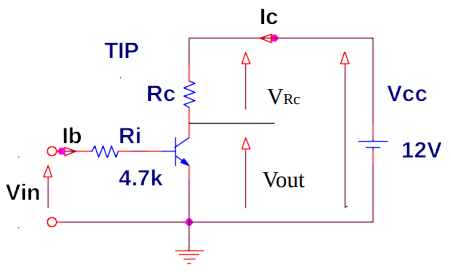
\includegraphics[width=0.55\linewidth]{Immagini/EXP7 - amplificatore.png}
        \caption{amplificatore BJT.}
        \label{fig: EXP7 - amplificatore}
    \end{figure}
    \item collegare in ingresso il generatore di funzione impostato su un'onda quadra di frequenza $\SI{1}{\kilo\hertz}$ e di ampiezza di qualche centinaia di mV sovrapposta ad un offset, questo deve essere tale si abbia $V_{ce}=\SI{6}{\volt}$ per $I_b$ costante;
    \item sovrapporre alla tensione di offset un'onda quadra molto piccola equivale a dare degli incrementi ad $I_b$. Ricavare con misure eseguite con l'oscilloscopio gli incrementi di $I_b$ e $I_c$
    \begin{equation}
        \Delta I_b=\frac{\Delta V_i}{R_i},\quad\Delta I_c=\frac{\Delta V_{ce}}{R_c},
    \end{equation}
    il cui rapporto fornisce
    \begin{equation}
        \beta_0=\left|\frac{\Delta I_c}{\Delta I_b}\right|;
    \end{equation}
    \item applicare un segnale sinusoidale e dal rapporto fra le ampiezze $V_{in}$ e $V_{out}$ lette sull'oscilloscopio calcolare l'amplificazione in tensione del segnale
    \begin{equation}
        A_V=\frac{V_{out}}{V_{in}},
    \end{equation}
    e verificare se è compatibile con il valore 
    \begin{equation}
        A_V=\frac{R_c}{R_i}\beta_0;
    \end{equation}
    \item Cambiare la frequenza di pilotaggio del segnale $V_{in}$ in ingresso e graficare $A_V$ in funzione della frequenza;
    \item Effettuare una regressione utilizzando come forma funzionale la funzione ricavata per il passa basso, aggiungendo un parametro che tenga conto del termine di amplificazione (guadagno maggiore di 1).
\end{enumerate}

\paragraph{Amplificazione di un'onda sonora (opzionale).} Collegare in parallelo alla resistenza $R_c$ un altoparlante e, mandando segnali di frequenza di circa $\SI{1}{\kilo\hertz}$, sentire l'onda sonora che si genera. Si può aumentare la frequenza fino alla frequenza di taglio dell'orecchio umano. Modulare il segnale in frequenza con lo sweep del generatore di funzioni e ascoltare l'onda sonora modulata.

\paragraph{Transistor in saturazione e interdizione (opzionale).} Osservare l'aumento della distorsione della tensione sinusoidale aumentando la tensione del segnale di ingresso fino ad avere il transistor in saturazione e in interdizione. Sostituire la $R_c$ con una lampadina e, facendo lavorare il transistor in saturazione ed interdizione, osservare che la lampadina si accende e si spegne (ovviamente se le frequenze di pilotaggio del transistor sono inferiori a $\SI{10}{\hertz}$).